As discussed in section \ref{sec:StateOfTheArt}, the TRITIUM monitor consists of a chain of three main elements, plastic scintillating fibers, that produce scintillating photons in response to a tritium electron decay, the photosensor, that detects the photons produced in the scintillator and produces an electronic pulse than gives information on the detected photons, and the electronic system, which processes and analyzes the electronic pulses provided by the photosensor. A scheme of a scintillation detector setup is shown in Figure \ref{fig:ScintillatorDetector}.

\begin{figure}[hbtp]
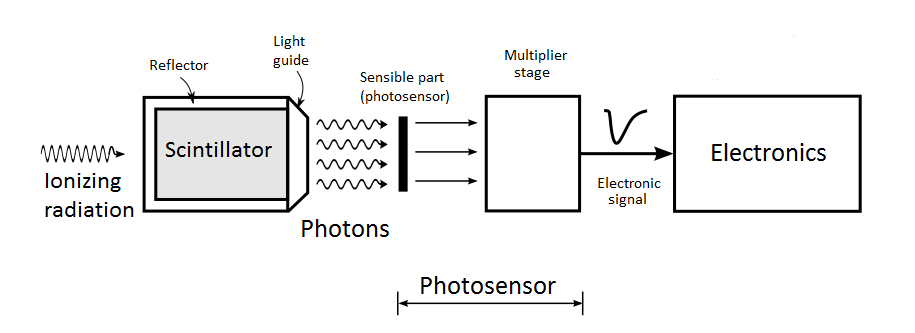
\includegraphics[scale=0.6]{3DesignPrinciples/32Tritium_detector/ScintillatorDetector.png}
\centering
\caption{Scheme of the scintillator detector.\label{fig:ScintillatorDetector}}
\end{figure}
